\chapter{IntroductionFrom  synapse}

\section{Importance}

Psychiatric and substance abuse disorders account for 7.1\% of disease burden as measured by disability-adjusted life years.\cite{murray2015global}.   A range of environmental and genetic factors are known to be implicated in their development. Of the genetic factors, most encode molecules that are found in the neuronal synapse, a structure that is responsible for the exchange and processing of information between nerve cells.

\section{The synaptic proteome - overview}

\subsection{Relevance to the thesis}
\todo{review and compress}
This thesis is about synapses and cognition. Specifically how the structure of the proteins making up synapses may affect the efficiency of cognition in man and model animals. 

The synapse is a complex system composed of thousands of proteins that form higher order structures.\cite{grant2012synaptopathies} To understand it I will use a network representation. I will then show how the network structure of synaptic proteins affects animal models of cognition and whether similar effects are seen in human population studies. 

This thesis will look at the structure of the protein interactions of the excitatory synapse and how these are related to animal models of cognition and genetic variations associated with differences in human cognitive ability in population studies.

\subsection{Synapses}
A nerve cell is composed of a number of dendrites that receive signals, a cell body or soma and an axon that transmits outgoing signals (figure~\ref{fig:soma and dendrites}). Between the axon and the dendrite are synapses (see figure~\ref{fig:synapse}).Synapses are junctions where information transfer occurs between nerve cells and are the most abundant structure in the brain \cite{grant2012synaptopathies}.

\begin{figure}
    \centering
    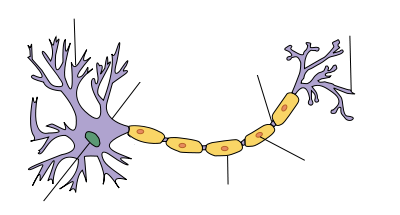
\includegraphics[width=0.9\textwidth]{images/Neuron-no_labels2.png}
    \caption{Soma and dendrites}
    \label{fig:soma and dendrites}
\end{figure}

Each nerve cell has an out outgoing axon but a cortical neuron receives input from around $10000$ synapses \cite{laughlin2003communication}\todo{check have checked laughlin check someone else}. Although synaptic numbers vary over time the number of synapses in the human neo-cortex has been estimated to be $1.5 \times 10^{-14}$ (0.15 quadrillion).\cite{pakkenberg2003aging}A synapse connects a presynaptic neuron and a postsynaptic cell across the synaptic cleft \cite{sudhof2012presynaptic}. The synapse is made up of proteins that self organise into macro-molecular machines that are responsible for signal transduction and processing.\cite{frank2016nmda}\todo{ref}  An essential function of the nerve cell is to integrate incoming information from the dendrites into a binary response at the axon.\cite{lassek2015synaptic} \cite{pocklington2006proteomes}

 The majority of synapses in the brain belong either to the excitatory glutamate system or the inhibitory GABA system. The most common type of synapse and neurotransmitter are the glutamatergic excitatory transmitters which comprise the main information processing system in the brain \cite{stewart2014structure} \todo{check ref}.

\subsubsection{History}
The term synapse, from the Greek ``to clasp together" was coined by Sherrington in 1897 writing in Foster’s textbook of physiology   Sherrington \cite{foster1895text} Since Cajal the principle model of the nervous system was of a structure composed of nerve cells built into higher order circuits. Prior to Cajal the brain was thought to be a syncytium. Cognitive complexity was thought to arise from an increasing number of connections.\todo{expand this section} 

\subsection{Molecular genetic revolution}
 Until relatively recently the synapse was thought to have a relatively simple structure controlled by a limited number of proteins and it was in the main a passive barrier across which neurotransmitters diffused.\cite{grant2019synapse}, \cite{lisman1994cam}  The brains functional unit was felt to the neural circuit and brain complexity arose from their pattern of connections. Synaptic function was limited to transferring information and maintaining a connection strength. This is not unreasonable as simple models of neurons can carry out complex calculations although they require weights at their connections analogous to synapses. This concurred with the model of learning which was that off increasing synaptic strength formalised by Hebb \cite{hebb1949organization_check}.
 
 Molecular interrogation of synaptic proteins became possible from 1992 with murine models. It was possible to catalogue synaptic proteins and clarify their function using knockdowns.  \cite{grant1992impaired}\cite{silva1992impaired}.  With the revolution in molecular genetics it was possible to characterise synaptic proteins. In 2000 Husi et al \cite{husi2000proteomic} identified 77 proteins in the NMDA receptor complex (NRC). In the next 5 years the number of synaptic proteins increased significantly, in 2006 an analysis considered the network of 186 proteins in the NRC-MASC complex \cite{pocklington2006proteomes}. The number of proteins in the post synaptic proteome as a whole had risen to 1124 in 2006\cite{collins2006molecular}.
 
 It soon became apparent that there were a very large number of proteins in the synapse and the synapse rather than simply being a gap for information transfer or a relay station was vitally involved in signal processing and computation as well as transduction. The number and combinatorial complexity of the proteins suggest an excess over what would be required for simply a connection weight.  Since 2000 the number of proteins found in synapses has greatly increased and it is now thought that there are over 3000 in the human although this number appears to be saturating. \cite{heil2018systems} \todo{query move this bit} The proteins that form the structure of the post synaptic area are modular and form higher order complexes\cite{pocklington2006proteomes}\cite{zhu2016mechanistic}\cite{frank2016nmda}.

\begin{figure}
    \centering
    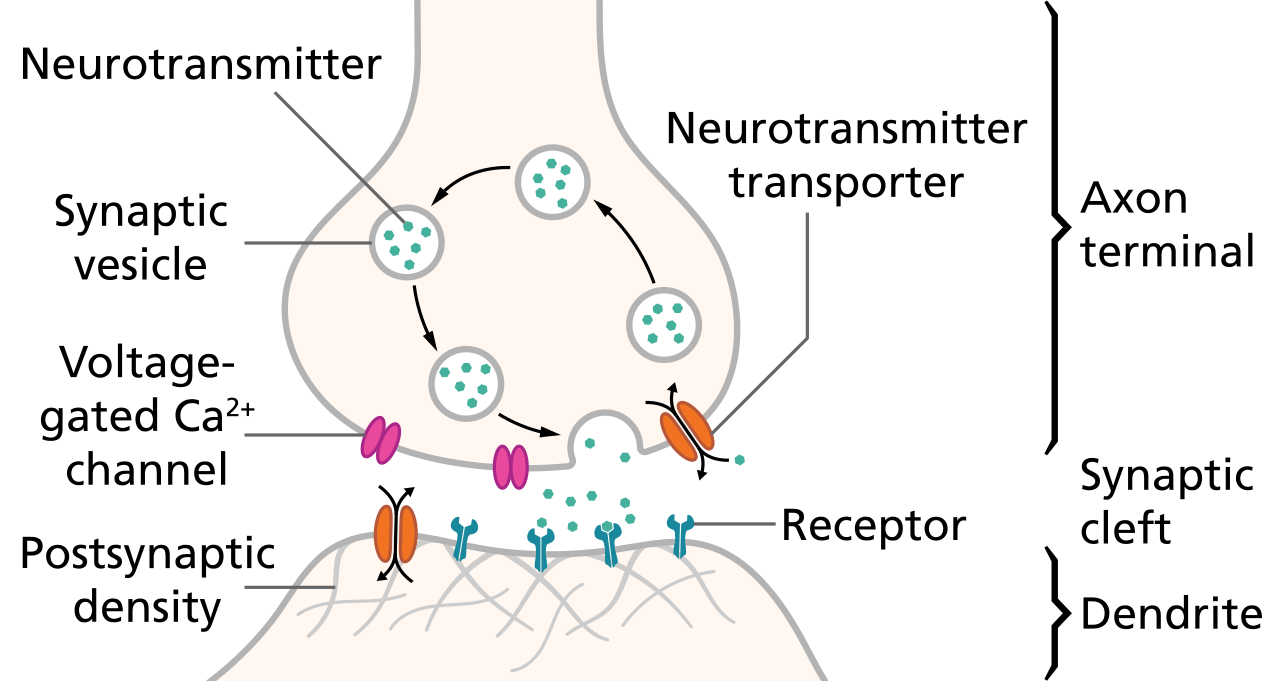
\includegraphics[width=0.9\textwidth]{images/SynapseSchematic_en.png}
    \caption{Schematic representation of synapse showing presynaptic area (labelled axon terminal) containing vesicles rich in neurotransmitters. Picture credit Thomas Splettestoesser Creative Commons \url{https://commons.wikimedia.org/wiki/User:Splette}}
    \label{fig:synapse}
\end{figure}



\subsection{Role in disease}
 

Bayes \cite{bayes2011characterization} identified 1461 proteins in human neocortical biopsies of the human post synaptic density (hPSD) and 748 that were consistent across three replicates. Using the Online Mendelian Inheritance in Man (OMIN) database \cite{hamosh2005online} and limiting the analysis to monogenic diseases the authors showed 269 diseases resulted from mutations in 199 hPSD genes and that 133 were primary nervous system disorders. Synapses are the source of action of many effective neuropsychiatric drugs and are central to putative disease mechanisms in psychiatric disorders \cite{thompson2015excitatory}, \cite{hu2015glutamate}. Also several psychotropic drugs with effects upon mood and perception have their mechanism of action at the synapse \cite{korpi2015mechanisms} as do other factors impacting on cognition and psychiatric health \cite{bocarsly2015obesity}. Reviews by Pocklington \cite{pocklington2014synapse} and Hall \cite{hall2015genetic} document convergent evidence for the importance of synaptic dysfunction in the aetiology of schizophrenia. 
The post synaptic density is the micro-molecular structure most implicated in neuropsychiatric disorders \cite{grant2012synaptopathies}. Evidence of its role in schizophrenia was found by\cite{focking2015proteomic} using proteomic studies of human brains. The evidence implicating the PSD, in particular the NMDA receptor complex, in exome sequencing of patients with schizophrenia is reviewed by Hall \cite{hall2015genetic}. Purcell et al. \cite{purcell2014polygenic} discuss the role of ARC proteins and calcium transport in schizophrenia. 
There is also evidence to suggest a role for glutamatergic signalling in Major Depressive Disorder (MDD).\cite{murrough2017targeting} \cite{de2017genetic}The anaesthetic ketamine has been extensively reported as having rapid onset efficacy in treatment of MDD. 

\subsubsection{High level function}

An important function of the synapse is controlling the strength of connections and cells that repeatedly fire at the same time are found to have strengthened connections (Hebbian learning)\cite{hebb1949organization_check}\todo{check ref. varies in references 1947 and 1949}. The discovery of long term potentiation by Bliss and Lomo \cite{bliss1973long} ultimately led to the discovery of the importance of glutamate transmission in LTP and the effect of disruption of synaptic proteins leads to a reduction in LTP and in learning
\todo{add in here or move from elsewhere the SG LTP heretical stuff}
A necessary component of adaptive neural information processing is modulating the ‘gain’ in signal from individual dendrites by controlling the strength of the connections between neurons. The synapse can do this through the processes of short and long term potentiation. Classical Hebbian \cite{hebb1949organization_check} long term conditioning requires the arrival of the signal at the presynaptic terminal, and postsynaptic depolarisation leads to a strengthening of connections.   Hebb posited a model where the strength of a connection between two neurons depends on how often they are activated together and as neural circuits determine behaviour these patterns of activation are then learned. Hebbian learning remains a fruitful model for computational models of learning. 

\section{Synapse structure}
The synapse is composed of a presynaptic area filled with neurotransmitter vesicles, a gap or cleft between the presynaptic areas and the post synaptic area and a post synaptic area containing neurotransmitter receptors and structural proteins. Nerve signals arrive at the presynaptic area, cause release of neurotransmitters from synaptic vesicles which diffuse across the cleft and are detected by post synaptic receptors whose activation may lead to depolarisation of the cell axon. 


\subsection{Presynaptic area}
The presynaptic area is separated from the post synapse by the synaptic cleft \cite{rusakov2011shaping}.  The synaptic cleft is approximately 20nm in size \cite{zuber2005mammalian}\todo{fix missing circumflex in first name of zuber} and is spanned by trans synaptic adhesion molecules.  \cite{missler2012synaptic}


 The presynapytic area contains neurotransmitters stored in vesicles which are docked and fuse with the plasma membrane at a specialised active zone an electron dense area , parallel to and juxtaposed to the plasma membrane.\cite{schoch2006molecular}. Neurotransmitters are substances which when they diffuse across the synaptic cleft give rise to signal in post synaptic receptor. Active vesicles are docked at the edge of the membrane and released following calcium influx. \cite{lassek2015synaptic}. After neurotransmitter release the vesicle is recycled by endocytosis.\cite{ashery2014molecular}
 
 Vesicles are primed by a protein complex consisting of 5 evolutionarily  conserved proteins acting as a complex RIM, Munc13, $\alpha$-liprin, RIM BP and ELKS proteins. \cite{sudhof2012presynaptic}. Piccolo and bassoon proteins are also associated with the active zone in vertebrates.  SNARE proteins facilitate vesicular fusion. \cite{sudhof2012presynaptic}. Mitochondria \cite{lassek2014proteome} are also an integral part of the presynaptic area and are noted on the earliest examinations \cite{gray1959electron}. The active zone is closely associated with extra cellular matrix \todo{ref}.
 
   In certain nerve cells such as photo-receptors, the active zone is ribbon like and capable of prolonged discharge  \cite{ashery2014molecular}.  
 
 Neurotransmitters transform nerve impulse signals through changing their pattern of release over short time frequencies in response to specific encoding of incoming signal (short term potentiation \cite{sudhof2012presynaptic}. Along with the post synaptic area they can strengthen the signal produced by neurotransmission over longer time scales (long term potentiation). A substantial amount of neural computation occurs in the presynaptic area and is dependent on synaptic proteins \cite{sudhof2012presynaptic}.
 
The presynaptic area developed from vesicle transport systems in earlier organisms and has developed more recently than the PSD.\cite{emes2012evolution}
 



\subsection{The post synaptic area and post synaptic density}

The post synaptic density (PSD) is an electron dense area parallel to the synaptic plasma membrane extending $\approx$ 35nm deep to the plasma membrane.\cite{harris2012ultrastructure} Formed from structural proteins that bind to actin in dendritic spines, and also to the receptor complexes, it contains protein kinases, receptor molecules and protein scaffold complexes such as PSD95. There are slight differences in its composition between mouse and man \cite{bayes2012comparative}, but in general its component structures are conserved in vertebrates.

Signal transfer across the synaptic cleft is typically mediated by neurotransmitter chemicals although direct electrical transmission can occur across gap junctions in the retina and in locations in the central nervous system.  \cite{stewart2014structure}\todo{cited by 11 see if we can find a better reference}. The neurotransmitter receptors are both held in place and modified by protein complexes such as guanylate kinases (MAGUK) that include glutamate receptors, and organise proteins involved in synaptic plasticity \cite{zhu2016mechanistic}. The release of glutamate is closely aligned with glutamate receptors in the post synaptic density (PSD). \cite{harris2012ultrastructure}

 The receptors in the post synaptic density show a geographical variation with the  $\alpha$-amino-3-hydroxy-5-methyl-4-isoxazolepropionic acid  receptors (AMPAR) and N-methyl D aspartate (NMDA) receptors in close apposition to the presynaptic active zone and the metabotropic glutamate receptors (mGluR) receptors in the peri-synaptic zone.\cite{scheefhals2018functional} 
 
 The ionotropic receptors have the fastest signalling characteristics and include NMDAR, AMPAR and Kainate receptors (KAR) named after the particular agonists found to provoke them.\todo{ref} Kainate acid receptors have a metabotropic G protein mediated element in their response and are less involved in synaptic transmission \cite{contractor2011kainate} than the two pure ligand gated inotropic receptors NMDAR and AMPAR.  The metabotropic glutamate receptor works through the mediation of g proteins and results in signalling and also recruitment of further ionotropic receptors to the post synaptic area.\todo{ref} \todo{does this not belong with the section~\ref{sec:Neurotransmitters} }
 
 The post synaptic density is the most evolutionarily ancient part of the synapse with its components arising in prokaryotes\cite{grant2018synapse} \cite{emes2012evolution}. 


The post synaptic proteins show many remarkable features. First they are relatively resistant to complete abolition of function.Even in knockout animals some signalling remains showing a degree of robustness, also dysfunction of many disparate elements result in common phenotypes particularly neuropsychiatric phenotypes. A very wide variety of mutations at different proteins and different loci within specific proteins can give rise to common disorders such as ASD. By contradistinction point mutations in key receptor proteins tend to give rise to severe phenotypes as we shall see later but also give rise to different phenotypes from mutations at different points in the protein (a case in point here being grin2a).

PSD proteins form into supercomplexes. 





\subsection{Molecular function}
Calcium ion influx is necessary for depolarisation. Synaptotagmin acts as a calcium sensor and allows for rapid fusion of synaptic vesicles with the cell membrane and release of neurotransmitters into the synaptic cleft.\cite{martens2007synaptotagmin}  It is also necessary for  learning in animals and long term potentiation and depression \cite{lisman2012mechanisms}.
\subsubsection{Neurotransmitters}
\label{sec:Neurotransmitters}
L glutamate , a small amino acid, is the dominant neurotransmitter at excitatory synapses within the brain \cite{niswender2010metabotropic}. Fast excitatory neurotransmission is carried out at the ionotropic glutamate receptors AMPA and NMDA \cite{traynelis2010glutamate}. Ionotropic glutamate receptors consist of 4 sub-units spanning the extracellular membrane that form a central ion pore. AMPA and Kainate receptors are homo or heterotetrameric but the NMDA receptor is obligatory heterotetrameric. The AMPA receptor is responsible for most of the fast excitatory transmission in the central nervous system \cite{henley2013ampa}. It is composed of four sub-units GRIA1-4 and is mainly permeable to sodium (Na+) and potassium (k) ions. The glutamate receptor sub-units originate from 18 different gene protein products representing NMDA, AMPA, Kainate and delta groups \cite{traynelis2010glutamate}. The NMDA receptor is also composed of four subunits (a tetrameter)  but is permeable to calcium ions. AMPA and KAR are fast acting working in less than 1ms \cite{traynelis2010glutamate} NMDAR depolarise more slowly in the 10ms range (cite neuron paper) 

Magnesium (Mg$^{2+}$) ions initially block NMDA receptor activity and  AMPA receptor activation is required to displace the Mg$^{2+}$ ions. AMPA is closely involved in long term potentiation. After Ca$^{2+}$ ion entry from the synaptic cleft, CAMKII is activated and leads to an increase in AMPA receptors at the post synaptic membrane.Calcium can entry through NMDA receptors after unblockage of Mg ions and its entry leads to activation of Calcium/Calmodulin dependent protein kinase. The kinase subsequently binds to NMDA receptors and phosphorylates sub-units of the AMPA type glutamate receptor.

Slow synaptic transmission, mediated by G protein second messengers, results from the action of metabotropic glutamate receptors \cite{niswender2010metabotropic} although mGluR signalling can also occur in time scales closer to igluR. There are eight mGluR subtypes. Metabotropic glutamate receptors are family C G Protein coupled receptors (GPCR). Group 1 mGLU promote intracellular calcium release whereas 2 are localised pre and post synaptically  and 3 are localised presynaptically \cite{niswender2010metabotropic} \footnote{grm 2,3,7 in group 5 - 2 and 3 are in group 2 , 7 along with 4,6,7,8 are om group 3, (grm 1 and 5 are group1), 1,2,3,5 and 7 are in the PSP, 1 is in 22 and 5 in group 32 - groups 20, 22 and 32 are quite closely related see \url{ source('~/RProjects/graph_groups/R/distribution_m_glu_glutamate.R')}Group II Metabotropic Glutamate Receptors Mediate Presynaptic Inhibition of Excitatory Transmission in Pyramidal Neurons of the Human Cerebral Cortex shows can be pre and post synaptic } but there is also evidence for pre and post synaptic action \todo{? more to discussion}
Metabotropic glutamaate receptors exert their effect by increases in protein synthesis Group II have been related to anxiety scz and alzheimers disease( Swanson) .
Glutamate levels are kept controlled by the glutamate glutathione pathway and glutamate transporters. 

\subsubsection{Long term potentiation}
Periods of synaptic activity can increase the strength of synaptic connections by the process of long term potentiation (LTP).

The theory that an increase in the strength of connection between neural cells leads to learning was first proposed by Cajal in 1911 \cite{nicoll2017brief}. Hebb proposed a model where there is synaptic modification following coextant pre and post synaptic activation \cite{hebb1949organization_check}. Later tetanic stimulation of rabbit hippocampal synapses was shown to result in an increase in the subsequnet strength of these responses.\cite{bliss1973long} NMDAR activity was subsequently shown to be necessary for LTP \cite{collingridge1983excitatory} but not for neurotransmission. 
 Interfering in the process of LTP in animal models leads to defects in memory and learning \cite{lisman2012mechanisms}).
 \cite{lisman2017glutamatergic} makes a connection between the modular structure of the synapse and the variety of potentiation responses.\todo{read this paper}`. The composition of the synapse into 70-80nm modules of independently activating AMPA receptors explains many problems with forms of plasticity.
 Six different forms of plasticity are observed in the synapse short term plasticity, long term plasticity, late long term plasticity, long term depression, distance dependent scaling and homeostatic scaling \cite{lisman2017glutamatergic}. Short term mpotentiation reuslts from weak stimuli and occurs early and is a promising model of working memory as GluA1 knockdown animals have abormal STP and long term memory. Early LTP is likely mediated by phospohrylation of GluA1 by CAMkII. Late long term potentiation is associated with a change in the size of the PSD. LTP is axiomatically defined as beginning 30 mins after a tetanic stimulus. Late LTP as associated with more AMPAR signalling with recruitment to the synapse and an increase in quantal probability. This often requires other factors such as dopamine in CA1 and BDNF and has been referred to as NeoHebbian. The mechanisms of this late stage include first increase in receptors from PSD 95 mediated \todo{check} CAMKII phosphorylation of stargazin or of syngap or activation of erk kinase through syngap. 
 MOdelling of the synapse suggests that responses can be explained if there are hotspots where there are either modules of AMPA receptor present or absent on vesicle release and plasticity can occur with recruitment to silent hotspots. \todo{network effects from this bit}
 
 
\subsection{The synaptogenic model of neural plasticity}


An alternative model of synaptic learning has been proposed that takes into account the level of synaptic complexity. In this model temporal neural signals are distributed according to the organisation of synaptic proteins into complexes and supercomplexes with specific combinations of elements attuned to particular temporal responses and then mapping to different areas in the brain. 

There are a number of reasons that the synaptic weight hypothesis may be incomplete, increases in LTP accompanied by difficulties in learning, very specific behavioural phenotypes from synaptic variation but without evidence of a circuit based change. 

 In contrast he suggests a bottom up synaptogenic model in which the synaptic protein composition acts as a zip code which allows spatially distributed neurons to respond to particular patterns of receptor stimulation. In support of his arguments he points out that the association of long term potentiation with learning remains controversial and it may be that the glutamate receptor (NMDA both subsume LTP and learning rather than affecting LTP which in turn causes learning. An example suggesting this is that mutations in PSD 95 give rise to cognitive impairments but increased long term potentiation.

\subsubsection{Analogy with synaptic models of computation}
\todo{commented out areas here may want to keep some of these}
% As regards the model of a bottom up approach to the structure of the synapse and behaviour we will adopt a similar approach seeking groupings of proteins and hence their cognate genes and seeing what their effect are on population studies of cognitive differences, enrichment for murine models of cognition or their role in disorders with a cognitive phenotype. Our approach however is looking for enrichment in-silico rather than in changes in behaviours of experimental model organisms. 

% One area I should mention here is that there is a middle ground between the one circuit one behaviour model with weights and a distributed bottom up model with an intrinsic frequency response. Primitive models of the synapse prove to be powerful computational devices. One of Grants arguments is that the synapse is a computational unit. A group of connected neurons with associated weights can give rise to complex decision making behaviour by allowing representation of structures being learned to be encoded as patterns more proximally in the network without there being a specific circuit for each response (for example in MNIST there is not a pattern of activation that is specific to 1 or 2 there are patterns of activation that are more likely to result in the final soft-max function choosing one of these) I would speculate that the combination of weights and circuits and the enormous complexity of the synapse allows to some extent the complex cognitive computations carried out by mammals particularly those in areas of locomotion and sensation that have proved so hard to simulate.
\subsection{Importance}

There are many reasons to be interested in synaptic function but I consider five to be of particular importance. 

First, synapses are involved in the overwhelming proportion of neuropsychiatric disorders \cite{grant2012synaptopathies}.  Second, they are composed of a large  number of proteins, many of which have roles outside of the nervous system and are an attractive basis to understand the genetics of complex cognitive traits, involving generalist genes, many of which exhibit significant pleiotropy \cite{sharma2000induction}\cite{plomin2015genetics}. Third, the synapse has proved a useful practical model of information processing and simplified models of the synapse have been able to carry out powerful computations \cite{hinton2007learning}, \cite{dean2012three}. However the synapse is considerable more complex than the simple weight used in these models. Fourth, synapses are the building blocks of higher levels of brain structures \cite{armstrong2012evolution} and will likely affect their function \cite{dean2012three}.

Finally they provide a molecular basis for human learning and memory \cite{kandel2014molecular},\cite{gallistel2013neuroscience}.
\section{The synapse}



      



\subsection{Evolution}


The presynaptic density has evolved earlier in evolution than the post synaptic density and is present from the time of the vertebrate expansion of the synaptic proteome. By contrast the PSP is more evolutionarily ancient. The proteins composing it are found in the earliest yeasts. The new proteins found in the mammalian PSP are the result of paralogue expansion. The PSP originated in the sensory signalling complexes of bacteria. These are too small to detect a difference in chemical gradient along their length and therefore Grant hypothesises that the function of these earliest receptors was to detect differences in chemical composition of their environment swim and then check again the composition of the environment. From this he concludes that the earliest function of the PSP is in recording differential pattern to the time course of signals arising in the organism. The presynaptic area is derived from endocytosis related mechanisms.

A genome duplication event approximately 550 Ma ago led to a significant increase in synaptic complexity \cite{nithianantharajah2013synaptic} , \cite{grant2016molecular}.

\todo{Cite those from extra bib also ? cite the Hill paper on evolutionary conservation much of this could go next to the pLI bit
}

Hill combined data from CHARGE and someone else to show using Linkage dysequlibrium regression. LD regression that areas of the genome enriched for SNPs associated with differences in intelligence were under negative evolutionary pressure finding these regions contained 2.6\% of SNPs but ~40\% of SNP based heritability. \cite{hill2016molecular} 

Networks as well as reduplication can provide robustness



 

\subsection{Systems Biology approaches to the synapse}

Systems biology entrails knowledge of the structure and dynamics of a biological system as a whole as well as its composite parts \cite{kitano2002systems}. System behaviour can differ from that of component parts and considering system structure, system dynamics, the control method and the design principle can help to understand these differences \cite{kitano2002systems}. Complex systems can be compactly represented as networks (section~\ref{sec:networks_intro}) and their structure analysed using algorithms derived from graph theory. Advances in computation, databases and ontologies improve our ability to understand , model and reason about these systems. 
 
\subsection{Models of the synapse}

Initial yeast models of the synapse were of poor quality so data mining of the literature for interactions was required to develop effective and comprehensive static models \cite{pocklington2006proteomes},\cite{armstrong2012evolution}. Databases are now of better quality and use standardised ontologies to organise their information)\cite{brazma2006standards}, \cite{hermjakob2004hupo}, \cite{kerrien2007broadening}. Databases however contain evidence on interactions that are less likely to be valid than evidence of direct experimental, interaction (eg literature data mining and co-expression). In order to develop a useful model of synaptic interactions, a significant amount of data cleaning, organisation and transformation of these databases is still required. This review will concern models where the interactions are inferred from experimental evidence of direct interaction in mouse or human. Synaptic components are purified using centrifugation and protein components examined by mass spectrometry. The process is reviewed in depth by \cite{lassek2014proteome} A comprehensive review of systems biology models of the synapse and their development is provided by Armstrong and Sorokina (2012). \cite{armstrong2012evolution}

\subsection{Static methods}

Protein-protein interactions in the synapse can be represented as an interaction graph with dots (vertices) representing the proteins and an edge connecting the vertices if the proteins interact. Alternatively the gene that encodes the protein product may be used. This is helpful if we wish either to annotate the structure with results from the biomedical or experimental literature, or to use the graph structure to better understand results from population molecular genetics. 

\subsection{Dynamic models}

Synapses can be modelled as dynamic entities with interactions between components and specific location, stoichiometric and kinetic constraints. Two common types are those based on systems of partial differential equations or agent based models. \cite{sorokina2013simulator},\cite{sorokin2014rkappa}, \cite{walpole2013multiscale}.

Although this thesis will not address dynamic models the interaction logic of the static model is essential for the generation of dynamic models. In addition if we discover structures within the network that have an enriched association with animal or population genetic models of cognition these will be fruitful areas for future dynamic simulation. 

\subsection{Finding communities in protein protein interactions}
Advances in molecular biology have increased our understanding of the function of the synapse and of its constituents. Initially the synapse was thought to be a relatively simple structure with few components but now there appear to be over 3000 proteins whose interactions are important for synaptic function. In addition there is a core of around 1000 proteins that are conserved across mammalian lines.  Protein interactions form macromolecular machines and the interconnections of proteins are vital to the function of the synapse. 
Synaptic proteins form modular structures \cite{pocklington2006proteomes} and there is evidence that the composition of these complexes are ‘optimally tuned’ for normal function \cite{grant2012synaptopathies}. Identifying and studying these large scale structures in the network may help in understanding the role of synaptic components in complex traits and neuropsychiatric disease.




\subsubsection{This is a bit about networks}
We have therefore a very complex wiring diagram of the synapse but we still don’t know what are its natural units and how the network structure of the synapse affects complex traits is unknown. One way to represent complex systems interactions is as a network. The burgeoning field of network science has made great advances this century and uses advances from graph theory, computer algorithms and statistical physics. Network theory allows the interrogation of the function of complex systems in terms of the pattern of their interconnections and shows common functional consequences of particular structures across disparate forms of network for example the internet, social networks and protein protein interactions. In this thesis I will show how an understanding of synaptic structure can help us to understand the molecular genetics of a complex trait in this case genetic differences in cognitive ability. I will also use the example of cognitive ability as a proof of concept of how these techniques can be used to understand neuropsychiatric disorders. Network approaches to disease

\subsection{Previous network based GSA}

\todo{citation error - could simply be that it is missing from the references}
\todo{PhD specific bibliography}
\cite{nguyen2018network}    review the use of pathway gsa for 36 packages.
Extends tools to 2017. If a package is not easy to use it will not be used by life scientists. Our approach makes use of commonly available GSEA and MAGMA packages and requires only editing of .gmt files which we provide software for. Of 45 packages, 30 were standalone or web based. They note that only one package is HIPPA compliant with web tools. Lots of the packages are implemented in R. Variety of ways in which information can be put in. If using list of genes this involves a cut off which involves loss of information. Discusses three different types of pathway signalling pathway, metabolic pathways and PPI. They note that SPIA accepts adjacency matrix representing a directed graph. Two types of graph models, single where a node is one thing and multiple. Topology GSA allows the graph to be split into sub graphs.
Then they discuss pathway scoring methods and the goal of producing a ranked list of pathways or sub-pathways.

\todo{Perhaps I should mention the use of david}

\subsection{Others not covered in this review}
Ghissian et al \cite{ghiassian2015disease}. There also appear to be other papers by Ghissian including on endophenotype. So for review this is the one where they use Louvain clustering on a generic network (? string) and find not \cite{blondel2008fast}so much but they fuind that the clustering of disease related genes together is greater than chance. he increasing evidence of the role of protein complexes mediating synaptic plasticity in schizophrenia.

The network can be analysed at the level of overall network, of an individual node or at the level of structures found within the network and I will discuss each of these with relation to cognitive ability. I will describe our experience of a pilot study and the reasons for choosing cognitive ability. I will also introduce and review the network analysis techniques that we utilised. 
 






\section{Intelligence}

\subsection{Measures and heritability}

People differ in their cognitive abilities and their ability to solve mental problems. The approaches to testing intelligence or cognitive abilities have been informed by function or lesion studies in the neuroscience community and on correlation between disparate tests revealing latent factors in the differential psychology literature \cite{deary2014stability} (Deary, 2014).

Given a number of different tests of cognitive ability individuals who do well on one test will tend to do well on others, and hence there will be a correlation between these results. This correlation between performance over several categories is the general intelligence factor, g or ‘general intelligence’, described by Spearman in 1904  \cite{deary2001intelligence}(Deary,2001), \cite{deary2014stability}. This construct accounts for about half the variance in individual cognitive performances \cite{deary2009genetic}(Deary et al 2009). The g factor can be discovered from a variety of disparate cognitive tests using principal component or factor analysis or by using cognitive tests that ‘load highly on the general cognitive factor’ \cite{johnson2004just}(Johnson et al. 2004), \cite{deary2009genetic} (Deary et al 2009).

As well as general cognitive ability (g), there is a positive correlation in performance on similar tests that relate to factors representing cognitive domains such as memory, processing speed, vocabulary, reasoning and spatial ability \cite{deary2010cognitive}(Deary et al 2010). In addition crystallized intelligence (gc) and fluid intelligence (gf), identified as factors of g by Cattell and Horn, change at different rates over the life course. Crystallized intelligence is composed of features such as knowledge of facts, vocabulary and certain number skills and does not tend to deteriorated until old age in contrast with fluid intelligence which requires ‘on the spot processing’ \cite{deary2010cognitive}(Deary et al 2010),\cite{davies2015genetic} (Davies et al 2015).
The heritability of cognitive abilities has long been recognised since Galton (1865). The genetic influence on human intelligence has been estimated at between 30 and 80\% and the heritability of the g factor increased from 30\% in youth to 50\% in adulthood to older age \cite{deary2009genetic}(Deary et al, 2009). 
Cognitive ability is an attractive complex cognitive trait to investigate using a structural model of the synapse. It is highly heritable and we know that a large proportion of its heritability can be marked by single nucleotide polymorphisms. In addition it can be reliable measured quantitatively; has a positive as well as a negative extreme, and is normally distributed \cite{plomin2015genetics}(Plomin and Deary 2014). Finally we have evidence that synaptic components are involved in variations in human cognitive abilities. 

The fact that this trait is normally distributed with a positive as well as negative extreme is attractive as it reduces the effect of hub centrality lethality effects on essential genes resulting in severe effects but not directly relating to their function \cite{jeong2001lethality}(Jeong et al 2001). Hubs, genes or proteins with large numbers of connections to other nodes are disproportionately involved in severe phenotypes but less so in complex and polygenic traits \cite{bayes2011characterization}(Barabasi et al 2011a) Analyses of communities in network models of the synapse therefore frequently yield associations with cognition (particularly when testing for over representation of terms in the biomdedical literature) due to mutations of these genes producing pjenotype that are associated with severe intellectual disability or non viability in animal models. Pocklington et al \cite{pocklington2006proteomes} (2006a) found that intellectual disability, unlike other neuropsychiatric disorders associated with cognition were widespread in the genome and through the clusters tha he identified in the MASC complex.

Intelligence is stable over the lifespan, both in terms of the average of the measure and rank. The correlation is about 0.7 but may be higher as the full range of those tested are not seen in follow up \cite{deary2009genetic}(Deary et al, 2009). Those of higher intelligence do not have better cognitive ageing but are more likely to have habits such as exercise and education that predispose to successful cognitive ageing \cite{deary2014stability}(Deary, 2014). 

Twin studies (Deary et al 2009)\cite{deary2009genetic} show greater correlation in changes in cognitive ability over a lifetime for monozygotic than dizygotic twins.

\subsection{Cognitive epidemiology}

Cognitive epidemiology is the study of intelligence as measured by psychometric tests – as an associated of mortality, illness and health (Deary, 2010)\cite{deary2010cognitive}. The effects of differences in cognitive function in health outcomes have been recognised since the 1930s \cite{deary2007cognitive}(Deary and Batty, 2007).

A systematic review of nine cohort studies found that IQ in childhood and early adulthood was associated with lower mortality in middle and late adulthood Batty et al (2007).\cite{batty2007premorbid} Higher cognitive ability is associated with important outcomes such as educational achievement and occupational success.

It is possible that the effect on lifespan might be due to social factors that have a common effect on intelligence, but studies including and analysis of three twin registries supported a genetic effect to explain correlation between lifespan and intelligence (for example the correlation I stronger for monozygotic than dizygotic twins (Arden et al 2016).\cite{arden2016association} General cognitive function affects the incidence of psychiatric disorders (Wraw et al 2015).\cite{wraw2015intelligence} Hill et al (2015) showed, using linkage disequilibrium regression, a common effect of genetic variants on cognitive ability and mental disorders with different effects at different points in the lifecourse.\cite{hill2016age}

\subsection{The molecular basis of cognition.}

One approach to the molecular basis of cognition has been that adopted by the Gene to cognition group (Croning et al, 2009).\cite{croning2009g2cdb} This is a pathway approach of examining variations in MASC and other synaptic genes which are linked to changes in memory in experimental animals (Deary et al 2009).\cite{deary2009genetic}

Molecular genetic approaches need to determine whether there is an effect of genetics on the environment ie genetic mediating environmental change, or whether genetic effects alter individuals’ susceptibility to the effects of environment (Deary et al 2009).\cite{deary2009genetic} In addition, although less marked in recent years, genetic approaches to cognitive ability remain highly controversial. In describing a computational systems biology approach to cognition, although it may appear clear from this review, it is important to avoid the implication that this implies a computational model of mind or of cognitive abilities. 

\subsection{Genome scale molecular findings}

Until recently the largest GWA study of intelligence in children (n=18,000) found no variants of genome wide significance (Benyamin et al 2014)\cite{benyamin2014childhood}, (Plomin et al 2013)\cite{plomin2013common}. The use of educational attainment, which has a moderate correlation with intelligence, has permitted the use of large study sizes which have shown genome wide significant findings but effect sizes have been small. Recently cohorts with larger sample sizes such as CHARGE and UKBiobank have permitted the identification of variants with significant association with cognitive ability at the genome wide level. 

Genome wide complex trait analysis (GCTA) (Yang et al 2011)\cite{yang2011gcta} of GWAS studies has shown that common SNPs can account for about half the heritability found from twin studies. Davies et al (2011)\cite{davies2011genome}, using five cohorts in the Cognitive Ageing Genetics in England and Scotland (CAGE) consortium (see section 13 for further details) used GCTA (Yang et al, 2011)\cite{yang2011gcta} to estimate the proportion of crystallised and fluid cognitive ability accounted for by linkage disequilibrium (LD) between SNPs and unknown causative loci. The estimates were 51\% for fluid intelligence and 40\% for crystallised intelligence. Using data from the Cohorts for Ageing Research in Genomic Epidemiology (end p 16) (CHARGE) consortia (PSATY ET AL 2009).\cite{psaty2009cohorts} Davies et al. (2015)\cite{davies2015genetic} estimated the lower bound of the narrow sense heritability for variation in cognitive ability to be 0.29 and 0.28 from the two largest cohorts in the meta-analysis.

Davies et al (2015)\cite{davies2015genetic} found 13 SNPs of genome wide significance for cognitive ability in a meta-analysis of data from the CHARGE consortium (n= 53949) Using VEGAS to generate gene level statistics, one gene was found of genome wide significance: HMGN1. The genomic inflation factor ($\lambda=$)\todo{Complete} suggests a polygenic effect on the phenotype.

Davies et al (2016)\cite{davies2015genetic} recently reported a genome wide association of 112151 individuals from UKBiobank (Elliot and Peakman, 2008)\cite{bycroft2018uk} \cite{elliott2008uk}. The association between genotype and educational attainment and three cognitive tests: reaction time, memory, numerical reasoning was tested. Gene based statistics were calculated using MAGMA without a gene window \cite{de2015magma}(de Leeuw et al 2015a). 149 SNPs at three independent regions were significantly associated with verbal numerical reasoning. Gene based analysis identified 17 significant genes across seven genomic regions. These included genes associated with mitochondrial function (NDUFA6), septin 3 which is associated with Alzeimers disease and other genes associated with neurobiological pathways (e.g. ATXN3L). The proportion of variance explained by common genetic variants calculated by GCTA was 31\%.
For reaction time there were 36 SNPs of genome wide significance spanning two regions. 23 genes across 9 regions were found to have significant associations with reaction time. 

There were no genome wide significant SNPs for memory. 115 SNPs were identified that were associated with educational achievement. Gene based analysis identified 95 genes across 28 regions associated with educational attainment.

\subsubsection{Recent GWAS}
\todo{CTG and UKBB}
Sniekers \cite{sniekers2017genome} in 2017 reported a meta-analysis of 78308 of  individuals of European ancestry from 13 cohorts including UK Biobank (54119). 336 SNPs were discovered in 18 genetic loci. 22 Genes were implicated by gene location and MAGMA GWGWAS identified 47 genes at a genome level of significance. 17 of these were also found by SNP genetic loci. Only one gene set was found to be significant after correction for multiple comparisons GO: regulation of cell development using MAGMA GSA (adjusted p=0.03, p=$3.5 \times 10^{-6})$.\cite{de2015magma} The authors note that the four next most significant gene sets (although not significant after correcting an $\alpha$ level of 0.05 for multiple comparisons) are related to neural function. The authors report that 14 of 44 genes which had data from the GTEx consortium were differentially expressed in the brain.\cite{gtex2015genotype}.Further analysis by combining this data with high intelligence cohorts is described \cite{coleman2019biological}.

Hill \cite{hill2019combined} used multi trait analysis of genome wide association studies using summary statistics MTAG\cite{turley2018multi} to increase sample size to 248 482 from 199 242. They included summary statistics from Sniekers (n=78,308)\cite{sniekers2017genome} and the study of educational attainment by Okbay (n=329417). These were augmented using 120934 new UK Biobank participants (UK Biobank Participants in the other studies contributing to the analysis being excluded). The new UK Biobank participants from this study will be used for analysis in this thesis as Intelligence\textsubscript{Discovery} cohort. 

They found 187 genetic loci associated with intelligence involving 538 genes. Gene set analysis using MAGMA revealed enrichment for 7 pathways incluiding  neurogenesis, regulation of nervous system development, regulation of cell development, neuron projection, central nervous system neuron differentiation, synapse \textcolor{red}{significantly for us}, neuron differentiation and oligodendrocyte differentiation. 

Savage \cite{savage2018genome} reported in 2018 a meta analysis of 14 different studies of general intelligence. This was again dominated by UK Biobank n=195653) with a significasnt contribution from COGENT. They reported 205 genomic loci and 1016 involved genes of which 939 were novel. 

There are reviewed by Plomin and Stumm\cite{plomin2018new}.

\subsection{Educational attainment}
\label{sec:Intro Educational Attainment}

The use of educational attainment as a proxy for intelligence has allowed a great expansion in sample size in GWA studies \cite{plomin2018new} as educational attainment is routinely reported in a number of social science and other GWA. The correlation between educational attainment and intelligence is phenotypically 0.5 and genotypically 0.65 in a review articles by Plomin. \cite{plomin2018new} citing  \cite{rietveld2014common}. In their report of a meta-analytic GWAS of intelligence Sniekers et al used LD score regression to calculate the correlation of their sample with 14 traits.\cite{sniekers2017genome},\cite{bulik2015ld}. The strongest assocation was with educational attainment (r\textsubscript{g}=0.70).

Rietveld et al (2013) \cite{rietveld2013gwas} looked at educational attainment as a proxy for cognitive ability. He used a meta anlysis of GWA studies examining the binary variable of college attendance, and regressed the number of years of education against the genotype (Rietveld et al 2013c). The discovery sample was 101,069 individuals, and the replication cohort 24,490 individuals. A total of 126599 individuals underwent genotyping and summary SNP data has been made available on the Social Science Genetic Association Consortium (educational attainment) website http://www.thessgac.org/!data/kuzq8. Rietveld et al (2013c) found three SNPs of genome wide significance, and all measured SNPs accounted for 2\% in the variance of outcome.\cite{rietveld2013gwas}

Okbay et al \cite{okbay2016genome}(2016b) reported 74 loci associated with educational attainment in an expansion of the cohort used by Rietveld The discovery cohort was now 293723 individuals in size and the replication cohort carried out on UK Biobank, 101,069. Gene set analysis showed enrichment for synaptic components particularly SHANK2. (pg18)

The largest educational attainment study to date is of 1.1 million individuals \cite{lee2018gene} The study was conducted using years of education as a phenotype in individuals of european ancestry. The authors identify 1271 independent genome wide SNPs. The authors were able to explain 11\% of educational attainment vairance using a polygenic risk score \cite{lee2018gene} \todo{this is quite close to the original although cited}. Using DEPICT they were able to show enrichment for pathways involved in the nervous system. The authors performed an analysis to support their depict findings using MAGMA GSA, interestingly they used a 5kB window around genes.  

Plomin (new) \cite{plomin2018new} box 5 makes the point about the availability of summary statistics and the non availability of some from commercial enterprises an observation which I completely agree with maybe should move to discussion.

\subsubsection{Recent GWA}
UKBB Ed and EA2 and overlap between and EA3

\subsection{Relevance to the systems neuroscience of the synapse}

The genetic architecture of differences in cognitive ability as of all complex traits, (to the extend that we can extrapolate from current studies), is that the genetic contribution to the phenotype is from many genes of small effect (Plomin and Deary 2014). In addition many of these genes are pleomorphic, shown by their association with health outcomes (Deary, 2008) and psychiatric morbidity (Hill et al, 2015). We have seen evidence that genes encoding synaptic proteins may be associated with cognitive ability and educational attainment (Hill et al 2014), (Okbay et al, 2016a).

Intelligence as the manifestation of the integrated function of neural systems is ‘central’ to systems neuroscience approaches (Plomin and Deary 2014), (Deary, 200). Network studies as we have discussed earlier, have implicated subsets of synaptic genes in intellectual disability and disorders with a cognitive phenotype (Pocklington et al, 2014), (Pocklington et al 2006a), (McLean et al. 2016). There is compelling evidence that the genetic effects on complex traits may be medicated by communities of genes (Barabasi et al, 2011a). I will discuss later (section 7.4) how network structure might allowed a relaxation of constraint in variation amongst many synaptic genes to produce a complex, continuous rather than severe phenotype.

I will describe a quantitative method that uses the large scale structure of networks to identify many genes of small effect which, acting in concert, may have an effect on cognitive ability. I will now consider how we can generate these communities before turing to the issue of how we will tedst their association with cognitive phenotypes.


We can extend this to multiple groups by recursively partitioning the network based on the leading eigenvector of the partiion and stopping partitioning when the partition does not result in a further increase in the modularity for the subdivision of the community (see Newman (2006) for further degtails). This is the method implemented by McLean et al (2016)

\subsection{Usefulness of intelligence as phenotype}

Before going on to discuss the methods that we can use to identify coherent sets of genes in a network we should point out that one of trhe aims of the study is to assess how well network analysis and clustering helps in the understanding of a phenotype. If the phenotype is poorly defined or their is a great deal of inter observed variability it may be that the clustering is measuring the phenotype (for example finding an unexpected subgroup of the phenotype) rather than assessing the effectiveness of modules of proteins associated with the phenotype.

\section{Gene level tests}

Genome wide association studies test the association of single nucleotide polymorphisms with a phenotype.
In order to test hypotheses about communities in the synaptome or perform tests such as gene set enrichment analysis for synaptic modules, it is necessary to reason at the level of vertices in a graph. It is necessary therefore to have a statistic for the significance of the association of a gene encoding a protein in the synaptome with a phenotype. This will require assigning SNPs to genes and generating a combined statistic (Petterson et al 2011).
Several authors have described methods for generating gene level association statistics. It has severl attractions. For one the num,ber of statistical testrs in doing inferecnnce is redeuced from over 500,000 for SNPs to approximately 20,000 for gene level tests with a commensurate reduction in the penalty for multiple testing. In addition genes are a natural biological unit and can be used in models of networks, proteins and other biological entities. Any form of pathway analysis will depend on finding a way of producing gene level statistics that are computationally tractable, reliable, repeatable and in which the analysis can easily be reproduced. As this will form the basis of our interrogation of netwroks, it is important that these foundations are sound. Given the lack of reproducibility in some computational approaches, particularly within network and pathway studies (Mitrea et al 2013b),. we (end p 34)
wish to ensure we can compare our findingsw with published work given a specific set of GWAS results.
This is rather problematic as many authors have used the WTCCC Crohns dataset to test simulations including de Leeuw et al (2015b), de Leeuw et al (2016), Li et al (2012), Li et al (2011) and Kwak and Pan(2015). Unfortunately this data is not available for donwload from the WTCCC website at present and when I wrote to the WTCCC they confirmed to me it was unavailable. Rietveld et al (2013c) uses data that is now publically available and quotes the gene level results from the software package VEGAS in the extended materials in his paper. It would seem reasonable that if we can reproduce these and show similarity between these results and other techniques we can assume that they are resonably reliable.

pFig 19 compares the results published in the supplementary materials from Rietveld et al (2013b) with those obtained running VEGAS on the data from this trial downloaded from the Social Science Genetic Consortium website. \footnote{Crohn's sets now}

\subsection{Assigning SNPs to genes}

The simplest approach is to use the top scoring SNPs in a gene (Wang et al 2007). This however canm be biased by gene size. Curtis et al (2008) suggested combining p values using Fishers combination test, but this assumes that the p values are independent which would not be the case in the presence of LD. Yang et al (2009)
suggested using the truncated p value test but this is also sensitive to the assumption of independence. 

The 'gold standard' used for comparison in the papers introducing most of the packages is the set based test in PLINK (Purcell et al 2007), which permutes phenotype labels for a set of SNPs to achieve a null distribution. To perform this for all SNPs in all genes is prohibitively computationally intensive and most methods use an approximation or asymptotic distribution to improve computational efficiency. In addition the set based test requires genotyped data, and several methods can now make use of summary statistics \footnote{want to use summary statistics as 1) rapid prototyping of methods by others 2) you can check the results}. I will consider the two implementations of VEGAS and MAGMA in more detail(end p35)

\subsubsection{Discarded SNPS}
Mention here or in the discussion that we are discarding approximately 50\% of SNPs that are not within protein encoding regions. 

\subsection{VEGAS}
VEGAS (Versatile Gene Based Association Study) was used to generate the gene level statistics in the study by Hill et al (2014) of gene set enrichment analysis \footnote{the other reason you want to keep GSEA in is future proofing - the methods are pretty clear and they are reported in a number of papers with pretty open implementations eg R gsea and all you need is the log10 p values of the gene score wheras with MAGMA the software changes anyway you don't want to put all of your eggs in one software basket - VEGAS was very very popular for a while then vegas 2 now not updated so much i think} of differences in cognitive ability. Liu et al. (2010) describes a method where the p values are converted to an upper tail chi square statistic with one degree of freedome. The pairwise LD vlues for all SNPs are calculate using \texttt{PLINK} with HapMap pahse 2 as a references population. VEGAS simulates draws from a multivariate normal distribution with mean 0 and covariance $\Sigma$, by taking the product of $n$ independent standard normal with the Cholesky decomposition of the LD matrix. This generates a correlated multivariate normal and is a common technique in Monte Carlo simulation (Murphy,2012) p817 and is the method implemented for generating correlated random numbers in \texttt{MATLAB}. The empricial distribution of the test statistic is compared with the draws from the multivariate normal to generate a p value. The progran is implemented in PERL and uses R to generate multiple draws from the nomral distribution and the R package corpcore (Shafer et al, 2013).
VEGAS represents a considerable increase in efficiency over the set test in plink but to generate gene base p values from a genome wide association study involves a running time of 18-30 hours. This can be problematic if the server is reset. The directory structure is very rigid and one cannot change the reference dataset or the build (to my knowledge). 

Its advantage is that it is simple to use and data is available for the 25 genes with highest p bvalues for gwas summary statistics that are publically available (Rietveld et al 2013c) \footnote{This is now true of magma with the results from ctg} It has also been widely used and its relative lack of options means one can compare results to other published genetic studies of cognitive abilities such as Davies et al (2011), (Hill et al 2014) and (Rietveld et al 2013a). While its runnning time is fast in comparison to the set test in \texttt{plink} the typical running time for a contemporary GWAS is 18-30 hours in my personal experience.

VEGAS 2 (Mishra and Macgregor, 2014) uses 1000Genomes rather than hapmap as the reference population and permits the use of gene windows of varying sizes but otherwise implements the same methods and has a comparable runnning time to VEGAS.

\subsection{MAGMA}
\label{sec:MAGMA_gene_scores}
\todo{Ask Douglas what of this should be methods}
MAGMA generates a gene based statistic using a multiple regression rather than a simulation model \cite{de2015magma}. Using summary gene data MAGMA uses either the mean $\chi^2$ statistic or top $\chi^2$ statistic to generate a p value. The mean method is the default and uses the properties of the sampling distribution.\cite{brown1975400} Top SNP scores can be calculated using a permutation method.   Linkage dysequlibrium is accounted for by using a reference population. 
 
% MAGMA projects the SNP matrix onto its principle components and removes SNPs with low explanatory power. The principle components are used to regress the pheotype in the gene level test. An F test is used to calculate a gene level statistic. 
MAGMA also includes a gene set test which tests the self contained hypothesis that the genes in the set have a greater association with the phenotype than all other genes. The gene p values are transformed into z values having a roughly normal distribution and reflecting the strengh of association of the gene with the phenotype. 

The gene set test uses a generalised least squares model where errors are the product of the variance and the gene gene correlation matrix $R$ which is calculated from reference data. Gene size, density and sample number are corrected for by treating them as covariates.
% to network communities I have not presented gene set tests for MAGMA but instead have used GSEA (Subramanian et al, 2005b). I have however used MAGMA to calculate gene level p values once I was able to confirm their similarity to the results of VEGAS because of the dramatically reduced runnning time (8-15 minutes).
% MAGMA allows the use of different NCBI genome assemblies for gene boundaries and uses 1000 Genomes to supply information on population LD.

For the work presented in this thesis gene level statistics were calculated using NCBI 37.3 build to provide gene boundaries and 1000 Genome European Ancestry to account for linkage disequilibrium. 

MAGMA has been widely used in the primary GWA studies of intelligence and cognitive ability and is the primary analysis method used in this thesis. This allows comparison of results with published MAGMA statistics. The results may vary slightly as the methods for calculating gene values are slightly different when raw genotype data is available. 

%For the work presented in this review, gene level statistics were calculated %using MAGMA and the NCBI 38 genome build \footnote{my !!! but the LBC data is %from VEGAS}. I have found that the results given by MAGMA aere on occasion very %sensitive to the genome build (see further work). My VEGAS data is incomplete %but should be finished in the next few weeks. I will also present MAGMA with %NCBI 37.3 as is used by Davies et al (2016) (see futher work).
\subsubsection{Remove}
\todo{? remove this bit}
MAGMA requires information on SNP chromosome and base location; where this is not available in summary data I have used SNP tracker (Deng et al, 2015).

MAGMA also has the attractive feature of preducing results as the Entrez id or HGNC gene symbols. It is useful to use the entrez id as it is used as the vertices in the models generated in igraph and is less susceptible to change than HGNC.
\subsubsection{Windows}
The use of a gene window significantly affects the number of SNPS assigned to genes. For example using the College Phenotype from Rietveld et al (2013c) of 2319112snsps 914887 were mapped to genes (39.45\%) using no window and NCBI37.3 build. 1385602 (59.75\%) mapped to genes using a 50kB window. (end of p 37)

\textcolor{red}{added}
Various window sizes are used \todo{bring together window bits}. \cite{zhao2017gene} use a 15kB window in a study of gene level statistics using the GATES method \cite{li2011gates} across psychiatric disorders as 90\% \cite{pickrell2010understanding} of eQTL are found in this region. 
FUMA uses a default 10kB window but this can be altered \cite{watanabe2017functional}. 
 
Figuere 9 Comparison of VEGAS and MAGMA


\begin{table}[h]
    \centering
    \begin{tabular}{llcc}
    \toprule
    Name     & Test & Year & Citations \\
    \midrule
    MAGMA     & F & 2015 & 665\cite{de2015magma} \\ 
    FUMA & MAGMA & 2017 & 426 \cite{watanabe2017functional}\\
    VEGAS2 & MonteCarlo & 2015 & 147 \cite{mishra2015vegas2}\\
    VEGAS & & 2010 & 743  \cite{liu2010versatile} \\
    FAST & GATES & 2013 & 36 \cite{chanda2013fast} \\
    \bottomrule
    \end{tabular}
    \caption{Comparison of Gene level scoring methods for summary GWAS statistics}
    \label{tab:gene_tests}
\end{table}
Figure 9 shows a comparison of the $-log10$ transformed $p$ values of VEGAS2 and MAGMA for the CHARGE data. $R^2$=0.98 \footnote{quote correlation} Image from compareMAGMAtoVEGAS.R. The results appear similar and it appears reasonable to compare results from MAGMA with the results provided from the study by Hill et al. (2014)
\subsection{PASCAL}
Lampterer et al \cite{lamparter2016fast} report the results of a method for using summary GWAS statistics to both generate gene level scores and do gene set analysis. The gene set analysis avoids the requirement for a cutoff and so can include contributions from low scoring genes. It provides similar scores to VEGAS in a shorter time scale and combines max of chi square (MOC) where the top scoring SNP is used and SOC (sum of chi square). Linkage dysequilibrium is accounted for using a reference panel (1000G) and information on LD is incorporated into the Gene Set Analysis score. Fishers method is used for 

Reports good similarity for VEGAS for genes with P score above $10^{-6}$ but with a marked increase in speed compared to VEGAS.

This thesis aims to give a general method for performing network analysis for complex traits involving the synapse. Therefore I have chosen to use two methods of gene scoring to avoid the dependence of all subsequent inference on the accuracy of gene scoring software. Although not as widely cited as MAGMA, PASCAL is widely used and has been used in a number of important GWA analysis. \todo{add citations} \todo{mention some of these papers} 

\subsection{Limitations of gene boundaries and non coding SNPs}
A number of SNPs are found in non coding regions of the genome. They may effect gene expression through affecting quantitative trait loci but these are excluded from analysis. For most analysis the discarded SNPs amount to about 50\%.

In order to include gene regulatory elements in gene level analysis a number of ``windows" around the gene boundary have been suggested both symmetric and asymmteric. VEGAS had a set 50kB boundary so some results such as Hill \cite{hill2014human} gene set analysis of the CAGES data set incorporate this. The predominant practice at present appears to be not to include a gene window or only a very small one of 5kb as per \cite{savage2018genome}.


\section{ Gene set tests}

Gene set analysis, also known as pathway analysis, tests the association of a set of genes with a particular phenotype. The set of genes can represent any grouping of genes based upon apriori biological knowledge. For example gene sets are often made up of the components of metabolic pathways, hence the synonyms pathway analysis. I shall be using communities discovered by community detection algortighms in graphs and subgraphs of the synaptic proteome as gene sets.

Gene set analysis was originally described in the contect of gene expression experiments (Mootha et al, 2003).

In gene expression analyses it can be difficult to obtain biological insight from such a large number of genes and no single gene may stand out against the background noise.

Carrying out inference over a set of genes increases power, allowing large numbers of genes of smaller aggregate effect to generate a detectable signal. It also provides a biological interpretation of a result of the tests in terms of a pathway or process (Subramanian et al 2005b). A variety of approaches have been described and their statistical properties are reviewed by de Leeuw et al (2016).

Gene set analysis (GSA) has been used with the results of genome wide association studies in conditions such as schizophrenia and multiple sclerosis (Jia et al 2010), (Jia et al 2011),(Consortium and Others, 2015) and in complex traits such as cognitive ability (Hill et al., 2014) and body mass index (Speliotes et al, 2010).

GSA tests can be divided into self contained tests, which test the hypothesis that the set is associated with a trait more than would be expected by change or competitive tests which test whether the set is more associated with the phenotype than the rest of the genome. An example of a self contained test would be Fishers exact test bassed on the hypergeometric distribution \footnote{is this right, also comparing to the entire genome verus a part of it such as PSP gives more significant results if for example you are looking at neural tissue)}. An example of a competitive test would be the test provided as part of the MAGMA suite (de Leeuw et al 2015a)

The most commonly used test judging by citations is Gene Set Enrichment Analysis Subtamanian et al (2005b)and was used by Hill et al (2014) to investigate enrichment of synaptic components for human cognitive differences. It is provided by the Broad Institute along with a variety of gene sets. de Leeuw et al (2016) considers GenGen Wang et al (2007) which is similar to GSEA in using a Kolmogorov Smirnov test as a self contained test \footnote{Original footbote: although it is not clear to me why and has the advantage of being non parametric}

\subsection{Komogorov Smirnov test}

The gene set enrichment analysis technique described by Subramanian et al (2005a) is based upon the rank ordering of sets of genes expressed in a phenotype and thos not of the phenotype, for example genes expressed in tissue that has been injured and those in tissues that have not been injured. An excess of expression of a set of genes, shown by a higher rank order of genes in the gene \footnote{sic}, is sought within the phenotype with the null hypothesis being that there is no difference between the two groups. The technique as described by Subramanian et al (2005a) uses the Kolmogorov Smirnov test to distinguish between the two groups. 

The Kolmogorov Smirnov test is a statistical test that compare the 'goodness of fit' of two probability distributions. The intuition behind the use of the test can be seen if we consider a random walk along one dimension. As the size of the walk steps tend towards zero and the number of steps increased towards infinity this becomes a continuous walk in time, a (end p 39)

Weiner process, $W(t)$. The maximum displacement of a random walk is proportional to $\sqrt{n}$where $n$ is the number of steps. When the beginning and end of the random walk on the alttice (or rel line) are bounded at the beginning and end of the process at zero, this becomes a Brownian bridge.

If we consider the cumulative distribution function (CDF) of any probability distributiobn the ends of the distribution are boubnded at 0 and 1. Therefore the difference between any two distributions CDF will be bounded at the start and end at 0. This can bve used to compare an empirial cumulative distribution function with that of known probability distribution. The maximum deviation from zero of the differecne between the two CDFs will approximate a two similar a random walk if they are similar the more different the distributions are the greater will be tmaximum difference between their CDF.

The Kolmogorov distribution describes the probability that the supremum of the Brownian bridge will take on a particular value. In the Kolmogorov Smirnov test the supremum of the distribution is used as the test statistic with the null hypothesis being that there is no difference between the distributions. In the case of gene set enrichment anlysis we are comparing the CDF of two empirical distributions (Clark and Ma'ayan,2011).

If we rank the genes of a microarray experiment in terms of their expression we will get a list. We have an apriori agreed set of genes based on some relation for example member no higher up the ordered list of gene expression than expected by chance. If we have a count that starts at zero and we increase the count proportional to the size of our set and the gene list when we see a gene in the setr and if we subtract from the count a step proportional to the nyumber of genes not in the set then at the end of the list the count at the end of the list will be zero. If we see a lot of genes in our set early on in the list of gene expression there will be an early positive deviation of the test statistic and its supremum will be high. A null distribution can be generated by randomly permuting the phenotype labels. Correction for multiple testing (for example checking a large number of sets) is carried out using the Benjamni and Hochbery procedure (Hochberg and Liverman 1994).

\subsection{The GSEA software}

The GSEA software is implemented in Java and has a graphical user and command line interface. The input format for gene sets provided by the user is either a gene matrix file ,gmx or a gene matrix transpose file .gmt.

These consist of tab or space separated files headed with the set name and with the gene names along the columns or rows.\footnote{MAGMA uses gmt and also gmt is easier if you are using python and building them up by using a number and a hash to a list with the gene elements in in addition gmx is difficult to implement using a dataframe (which is what it looks like it is designed for) because dataframes require the same length.} The Broad Institute suggests using spreadsheet software such as Excel to generate the files (see methods) \footnote{include ref for the errors due to date} \footnote{also note in the intelligence literature ? have people used the full gmx list even although there is a high prior probability that they involve neural tissues what would be the result of the published studies if we only looked at gene terms that are neural USE NIGO set   Geifman et al}P values are reported for the gene sets based on permutation along with false discovery rate \cite{benjamini1995controlling}\footnote{describe FDR} and family wise error rate (Subramaniam et al 2015) , (Hochberg and Liberman, 1994).

\subsection{GSA with MAGMA}

\subsection{GSA with PASCAL}
\cite{lamparter2016fast}
\section{Networks}
\label{sec:networks_intro}
\subsection{Network effects}
One thing that was noticed early on was that not all knockdowns lead to complete loss of function \cite{keverne1997evaluation}. \cite{charlesworth2016canalization}
\section{Random graphs}
\label{sec: intro_random_graphs}
\section{Centrality measures}
\label{sec: intro_centrality_measures}
\section{Community detection}
\subsection{Rejectedalgorithms}

I have tested some other available algorithms for community detection, many of which are in wide use. The parallelised implementation of Geodesic and Random Edge Betweeneness algorithms (Newman and Girvan, 2004) implemented by McLean et al failed to complete after two days when dealing with the large num,ber of vertices in the synaptome ($>4000$ vertices).\cite{mclean2016improved}

Louvain \cite{blondel2008fast} community detection is widely used, works at scale and has been most widely applied in the analysis of large scale social networks. It is a greedy optimisation method to optimise modularity. 
Blondel et al (2008) compares this with other community detection algorithms and finds that this algorithm has the lowest running time and maximises the increase in modularity.
Using the algorithm to detect communities in the synaptic proteome failed to generate communities that 'looked right' and the communities did not enriched for any phenotype in the gene set analysis.

The greedy implementation of a modularity maximisation procedure that is said by Kolacyzk and Csardi (2014) to approximate Newman and Girvan (2004) in igraph (Csardi and Nepusz, 2006) was rejected for identical reasons. A review of the performance of igraph algorithms is presented by De Souza and Zhoa (2014). (end p 33) \footnote{to do try to find the multilayer louvain implementation}

\subsection{Spin glass}

I graph implements a spin glass algorithm where the communities are represented as a Potts spin glass model, a generalisation of the Ising two state model where the spins are communities. Community detection corresponds to minimising the Hamiltonian of the Pott's model (Eaton and Mansbach, 2012). I have used this model to produce communities of constrained size. I have not yet tested these communities in the replication cohort (CHARGE) and they are not presented in this review (see further work section 18.8) \footnote{spin glass other gamma and Coin has not used max spins which limits community size}.

\subsection{Problem of singletons}

The spectral clustering algorithm has a tendency to produce isolated nodes. This problem is more marked on sparse networks and difficulties with sptreacl partiioning in sparse networks is well recognised (Krzakala et al.,2013). On occasion these 'singleton' communities in combination contribute a significant amount of the genetic signal found inm the graph. I have written a script to collect singletons into sets and test these but this data is not presented here. I discuss the problems of singletons in further work (section 18.8)

\section{Using network topology}

The gene sets in gene set analysis are often portions of pathways and pathway analysis is often used synonymously with GSA. Some authors however have used the term to refer to analysis, where the topology of the pathway or graph is part of the analysis but the terms are used inconsistently.

Khatri etr al (2012) reviewed pathway analysis methods and identified three methods. Over representation analysis,k functional class scoring, and pathway tology or third generation methods.

Mitrea et al (2013a), reviewing topology based methods, notes that several techniques that claim to be third generation methods use the pathway topology to provide what is essentially a gene set (ie a pathway or portion there of from KEGG or a similar database) and so exclude information on pathway structure topology. Mitra et al (2013a) criticised Khatri et al (2012) for including methods including functional analysis and annotation with Gene Ontology terms as 'third generation' analysis methods.

Barabasi et al (2011b) reviewed a number of methods that used netowrk based statistics such as clustering coefficient to augment the analysis of gene expression oand GWAS studies. Of particular interest is the use of a 'disease community' which I will return to in further work. 

Pandey et al. (2012) reports using eigenvector centrality of SNPs within a pathway to prioritise genes for pathway enrichment. The edges within the network however refer to gene - gene interaction strength rather than network topology (Davies et al 2010) \footnote{perhaps I should mention WGCNA}.

Frost et al (2014) describes a spectral method for gene set enrichment but this refers to the principle component analysis of a snp matrix and a matrix of indicator variables referring to gene properties.

Mitrea et al (2013a) draws attention to the fact that the results of methods that actually use network topology are difficult to assess and compare. The review points out thtat it is often impossible to reproduce results even with the cooperation of the authors. A largee number of the packages are web based and inflexible in the networks that they use.

One reason is that MItrea et al (2013b) defines the goal of mpathway analysis using network topology: 'to identifiy the most significantly impacted pathways from a large collection of heterogenous pathways'. A difficulty with this is that there is no natural boundary between pathways or subgraphs of pathways making the possible sets being tested very large. In addiiton the 'most significantly impacted pathway' is not always definitively identified by these methods.  (end p 41)

This is perhap best explained by reference to two of the most widely cited of these tools, both by the same author. 

Glaab et al (2010) describes topoGSA, one of the more widely used packages. For a given gene set it calculates network parameters such as degree, local clustering coefficient, shortest path length, node betweenness and eigenvector centrality along with a Fisher;s exact test for pathways which contains genes in the set in KEGG, Interpr, BioCarta or Gene Ontology and with the network data provided by querying the STRING database. An overal similarity score is provided based on the sum of ranks. For an explanation of network metrics see section 7.4.

It has an easy to use web interface but the user must decide on a cut off significance level and no use is made of the ranks of the genes in the set. Results from topoGSA are shown in figure 10 and figure 11 using publicly available data used in this study.

Figure 10 TopoGSA network enrichment program. The set usied in this example is the list of NMDA receptor genes from Hill et al (2014). end p42

Figure 11 Topo GSA network enrichment program. The edxampe set is the top50 Genes from Okbay et al (2016b)

The approach is interesting but is limited by the factors that limit the use of Fisher's exact test. The use of network statistics at an individual level for cognitive abilities show no correlation with gene $p$ value for the CAGES data set \footnote{nor for the later datasets}. The authors do not record if the use direct interactions, or interactions based on techniques such as literature data mining, which are available in STRING. Finally the web based interface makes it improactical for large scale analysis of GWAS data. It is essentially a, a tool for exploratory gene expression analysis and it is not clear that it has an advange over GSEA using the BROAD institute's MSigDB database (Liberzon et al 2011). 

The enrichnet package by the same author (Glaab et al 2012) makes greater use of network topology, calculating a distance metric between the gene sets and the STRING (end of p43)

database, using a random walk with restart (Xd distance). This is compared to the result of Fisher's exact test. Once againm this is in essence a reweighting of Fisher's exact test, to identify a potential netowkr. It may hold an advantage over GSEA but I found it hard to interpret the significance of its results other than augmenting the intepretation of Fisher's exact test with a measure of network closeness.

It is relatively widely used with 87 citations \footnote{check}. The use of random walk to make a sample of a particular netowrk is interesting \footnote {it will to some extent do the same thing as community detection ie if you are in a community you will tend to stay within it and I will return to this in section 18.8 (heading speculative work)} \footnote {how easy is it to export and repeat these anlayses}

Figure 12 - Enrichnet gene set enrichment pacakge. NMDA geneset from Hill et al 2014)

I propose an alternative approach would be to use the better understood process of gene set enrichment analysis and to use as sets the communities identified by a community detection algortihm. The setsw will be defined entirely by their network topology (see 8.1).
 You can also look at measures of centrality by separately testing their correlation with results of genes in experiment e.g. gene p  values or fold change
 To avoid problems due to heterogeneous or incomplete network data described (end $p 43b$) above we must use a high quality curated data set to construct the network model of the synapse 

\footnote{it is also important to use a tissue specific model as Barabasi showed that disease genes are more likely to be tissue specific rather than universally expressed and different proteins in a tissue will result in a different network}

\section{Network models}

Figure 13 Interaction graph of full synaptosome for direct published interactions. Nodes are genes, interactions are edges. Node size is proportional to degree. For high degree nodes please see table 4. Nodes 4612, edgess 16782 Layout forcetlas. Figure produced in Gephi 0.9.1 \footnote{we an look at the number of edges versus nodes over tme and with the Pocklington model and the one Colin had of the consensus PSD.}

The network modesl of the synaptic proteome were produced by the Synaptic-Proteome-Group (2016) for a forthcoming paper. The paper reports the state of the art in combininh disparate databases and primary proteomic data to produce a high quality representations of the synaptic proteome. 

The model is a static interaction graph of the genes that encode the protein components of the synaptic proteome. only those interactions for which there are direct experimental evidfence of interaction are included. The interactions are mined from protein interaction datbases usng the PSIMI format (Hermjakob et al,2004a). The largest component is from the union of HIPPIE (Schaefer et al,2012), Biogrid (Chatr-Aryamontri et al, 2015) and Intact (Hermjakob et al, 2004b) databases. The full network graph is shown in figure 13. end p45.

The interactions are recorded 

\section{Plan}
\label{sec:intro plan to procede to next chapter}

Need to include here: In order to investigate the effect of community structure and network structure in the PSP on a complex cognitive trait we developed a model of the PSP and derived a measure of the significance of a synaptic gene for a complex trait in this case intelligence and educational attainment using MAGMA GSA. To permit the use of a discovery and replication cohort study design in some subsequent sections of this thesis we obtained summary genetic data from 2 GWA of intelligence and 2 GWA of educational attainment. The next chapter describes the processing of this data and the generation of the interaction graph.
